% ------------------------------------------------------
% ------------------------------------------------------------------------
% abnTeX2: Modelo de Trabalho Academico (tese de doutorado, dissertacao de
% mestrado e trabalhos monograficos em geral) em conformidade com 
% ABNT NBR 14724:2011: Informacao e documentacao - Trabalhos academicos -
% Apresentacao
% ------------------------------------------------------------------------
% ------------------------------------------------------------------------

\documentclass[
	% -- opções da classe memoir --
	12pt,				% tamanho da fonte
	openright,			% capítulos começam em pág ímpar (insere página vazia caso preciso)
	twoside,			% para impressão em verso e anverso. Oposto a oneside
	a4paper,			% tamanho do papel. 
	% -- opções da classe abntex2 --
	chapter=TITLE,		% títulos de capítulos convertidos em letras maiúsculas
	%section=TITLE,		% títulos de seções convertidos em letras maiúsculas
	%subsection=TITLE,	% títulos de subseções convertidos em letras maiúsculas
	%subsubsection=TITLE,% títulos de subsubseções convertidos em letras maiúsculas
	% -- opções do pacote babel --
	english,			% idioma adicional para hifenização
	brazil				% o último idioma é o principal do documento
	]{abntex2}

% ---
% Pacotes básicos 
% ---
\usepackage{lmodern}			% Usa a fonte Latin Modern			
\usepackage[T1]{fontenc}		% Selecao de codigos de fonte.
\usepackage[utf8]{inputenc}		% Codificacao do documento (conversão automática dos acentos)
\usepackage{lastpage}			% Usado pela Ficha catalográfica
\usepackage{indentfirst}		% Indenta o primeiro parágrafo de cada seção.
\usepackage{color}				% Controle das cores
\usepackage{graphicx}			% Inclusão de gráficos
\usepackage{microtype} 			% para melhorias de justificação
\usepackage{hyperref}
\usepackage{trivfloat}
\usepackage{datetime}
\usepackage{graphicx}


%\usepackage{listings} usado pra colocar codigo


\trivfloat{quadro}





\usepackage{novacapa}
% ---
		
% ---
% Pacotes adicionais, usados apenas no âmbito do Modelo Canônico do abnteX2
% ---
%\usepackage{lipsum}				% para geração de dummy text
% ---

% ---
% Pacotes de citações
% ---
\usepackage[brazilian,hyperpageref]{backref}	 % Paginas com as citações na bibl
\usepackage[alf]{abntex2cite}	% Citações padrão ABNT

% --- 
% CONFIGURAÇÕES DE PACOTES
% --- 

% ---
% Configurações do pacote backref
% Usado sem a opção hyperpageref de backref
\renewcommand{\backrefpagesname}{Citado na(s) página(s):~}
% Texto padrão antes do número das páginas
\renewcommand{\backref}{}
% Define os textos da citação
\renewcommand*{\backrefalt}[4]{
	\ifcase #1 %
		Nenhuma citação no texto.%
	\or
		Citado na página #2.%
	\else
		Citado #1 vezes nas páginas #2.%
	\fi}%
% ---

% ---
% Informações de dados para CAPA e FOLHA DE ROSTO
% ---
\titulo{Thin client Raspberry PI}
\autor{Felipe Lima Morais}
\local{Dourados, MS}
\data{2015}
\orientador{Prof. Dr. Fabrício Sérgio de Paula}
\instituicao{Universidade Estadual de Mato Grosso do Sul}


\tipotrabalho{Trabalho de Conclusão de Curso em Ciência da Computação}
% O preambulo deve conter o tipo do trabalho, o objetivo, 
% o nome da instituição e a área de concentração 
\preambulo{Este  exemplar  corresponde  à  redação  final da
monografia da disciplina Projeto Final de
Curso devidamente corrigida e defendida
por \imprimirautor \  e aprovada pela
Banca  Examinadora, como parte dos
requisitos para a obtenção do título de
Bacharel em Ciência da Computação.}
% ---


% ---
% Configurações de aparência do PDF final

% alterando o aspecto da cor azul
\definecolor{blue}{RGB}{41,5,195}
%\definecolor{blue}{RGB}{0,0,0}

% informações do PDF
\makeatletter
\hypersetup{
     	%pagebackref=true,
		pdftitle={\@title}, 
		pdfauthor={\@author},
    	pdfsubject={\imprimirpreambulo},
	    pdfcreator={LaTeX with abnTeX2},
		pdfkeywords={abnt}{latex}{abntex}{abntex2}{trabalho acadêmico}, 
		colorlinks=false,       		% false: boxed links; true: colored links
    	linkcolor=blue,          	% color of internal links
    	citecolor=blue,        		% color of links to bibliography
    	filecolor=magenta,      		% color of file links
		urlcolor=blue,
		bookmarksdepth=4
}
\makeatother
% --- 

% --- 
% Espaçamentos entre linhas e parágrafos 
% --- 

% O tamanho do parágrafo é dado por:
\setlength{\parindent}{1.3cm}

% Controle do espaçamento entre um parágrafo e outro:
\setlength{\parskip}{0.2cm}  % tente também \onelineskip



\renewcommand{\imprimircapa}{%     CAPA MODELO DE CIÊNCIA DA COMPUTAÇÂO
\begin{capa}%
	\center
	

	\begin{tabular}{@{}c@{}}
	\toprule
	Curso de Ciência da Computação            \\
	\ \ \ \ \ \ \ \ \ \ \ \ \ \ \ \ \ Universidade Estadual de Mato Grosso do Sul\ \ \ \ \ \ \ \ \ \ \ \ \ \ \ \ \  \\ \bottomrule
	\end{tabular}

	
	
	
	\vspace*{\fill}
	\begin{center}
		\ABNTEXchapterfont\bfseries\LARGE\imprimirtitulo
	\end{center}

	\vspace*{\fill} 
	{\large \imprimirautor}
	\\
	\vspace*{\fill}
	\imprimirorientador
	\\
	\vspace*{\fill}
	{\large Curso de Ciência da Computação}
	
	Universidade Estadual de Mato Grosso do Sul
	\\
	\vspace*{\fill}
	
	\large\imprimirlocal \\
	\large\imprimirdata
	\vspace*{1cm}
	
\end{capa}
}



\makeatletter
\renewcommand{\folhaderostocontent}{
\begin{center}
{\ABNTEXchapterfont\bfseries\Large\imprimirtitulo}
\vspace*{\fill}\vspace*{\fill}
\begin{center}
\Large\imprimirautor
\end{center}
\vspace*{\fill}
\abntex@ifnotempty{\imprimirpreambulo}{%
\hspace{.45\textwidth}
\begin{minipage}{.5\textwidth}
\imprimirpreambulo \\
\end{minipage}%
\vspace*{\fill}
}%


\abntex@ifnotempty{\imprimirpreambulo}{%
\hspace{.45\textwidth}
\begin{minipage}{.5\textwidth}
	\begin{center}	
	Dourados, \today \\
	\end{center}
	\vspace*{2cm}
	\begin{center}	
	\imprimirorientador \\
	\end{center}
\end{minipage}%
\vspace*{\fill}
}%



\vspace*{1cm}
\end{center}
}
\makeatother






% ---
% compila o indice
% ---
\makeindex
% ---

% ----
% Início do documento
% ----
\begin{document}

% Seleciona o idioma do documento (conforme pacotes do babel)
%\selectlanguage{english}
\selectlanguage{brazil}

% Retira espaço extra obsoleto entre as frases.
\frenchspacing 

% ----------------------------------------------------------
% ELEMENTOS PRÉ-TEXTUAIS
% ----------------------------------------------------------
% \pretextual

% ---
% Capa
% ---
\imprimircapa %default antex2 





% ---

% ---
% Folha de ros
% (o * indica que haverá a ficha bibliográfica)
% ---
\imprimirfolhaderosto*
% ---

% ------------------------------------------------------------------------------------------------------------
% Inserir a ficha bibliografica
% -----------------------------------------------------------------------------------------------------------

% Isto é um exemplo de Ficha Catalográfica, ou ``Dados internacionais de
% catalogação-na-publicação''. Você pode utilizar este modelo como referência. 
% Porém, provavelmente a biblioteca da sua universidade lhe fornecerá um PDF
% com a ficha catalográfica definitiva após a defesa do trabalho. Quando estiver
% com o documento, salve-o como PDF no diretório do seu projeto e substitua todo
% o conteúdo de implementação deste arquivo pelo comando abaixo:
%
% \begin{fichacatalografica}
%     \includepdf{fig_ficha_catalografica.pdf}
% \end{fichacatalografica}

% 																Area comentada 
%\begin{fichacatalografica}
%	\sffamily
%	\vspace*{\fill}					% Posição vertical
%	\begin{center}					% Minipage Centralizado
%	\fbox{\begin{minipage}[c][8cm]{13.5cm}		% Largura
%	\small
%	MORAIS, Felipe Lima.
%	%Sobrenome, Nome do autor
%	
%	\hspace{0.5cm} \imprimirtitulo. \\
%
%	\hspace{0.5cm} \parbox[t]{\textwidth}{\imprimirtipotrabalho. \imprimirlocal. \\
%	\imprimirinstituicao, \imprimirdata.}\\
%	
%	\hspace{8.75cm} CDD: 02:141:005.7\\
%	\end{minipage}}
%	\end{center}
%\end{fichacatalografica}



% -----------------------------------------------------------------------------------------------------------
% Fim ficha bibliografica
% -----------------------------------------------------------------------------------------------------------



% -----------------------------------------------------------------------------------------------------------
% Inserir folha de aprovação
% -----------------------------------------------------------------------------------------------------------

% Isto é um exemplo de Folha de aprovação, elemento obrigatório da NBR
% 14724/2011 (seção 4.2.1.3). Você pode utilizar este modelo até a aprovação
% do trabalho. Após isso, substitua todo o conteúdo deste arquivo por uma
% imagem da página assinada pela banca com o comando abaixo:
%
% \includepdf{folhadeaprovacao_final.pdf}
%

%																	Area comentada
%\begin{folhadeaprovacao}
%
%  \begin{center}
%    {\ABNTEXchapterfont\large\imprimirautor}
%
%    \vspace*{\fill}\vspace*{\fill}
%    \begin{center}
%      \ABNTEXchapterfont\bfseries\Large\imprimirtitulo
%    \end{center}
%    \vspace*{\fill}
%    
%    \hspace{.45\textwidth}
%    \begin{minipage}{.5\textwidth}
%        \imprimirpreambulo
%    \end{minipage}%
%    \vspace*{\fill}
%   \end{center}
%        
%   Trabalho aprovado. \imprimirlocal, \imprimirdata:
%
%   \assinatura{\textbf{\imprimirorientador} \\ Orientador} 
%   \assinatura{\textbf{Professor} \\ Convidado 1}
%   \assinatura{\textbf{Professor} \\ Convidado 2}
%      
%   \begin{center}
%    \vspace*{0.5cm}
%    {\large\imprimirlocal}
%    \par
%    {\large\imprimirdata}
%    \vspace*{1cm}
%  \end{center}
%  
%\end{folhadeaprovacao}

% -----------------------------------------------------------------------------------------------------------
% Fim folha de aprovação
% -----------------------------------------------------------------------------------------------------------



% -----------------------------------------------------------------------------------------------------------
% Dedicatória
% -----------------------------------------------------------------------------------------------------------

%\begin{dedicatoria}
%   \vspace*{\fill}
%   \centering
%   \noindent
%   \textit{DEDICATORIA PRA QUEM QUISER} \vspace*{\fill} %TODO
%\end{dedicatoria}

% -----------------------------------------------------------------------------------------------------------
% Fim Dedicatória
% -----------------------------------------------------------------------------------------------------------



% -----------------------------------------------------------------------------------------------------------
% Agradecimentos
% -----------------------------------------------------------------------------------------------------------

\begin{agradecimentos}

A Deus por ter me dado saúde e força para superar as dificuldades.

Obrigado aos meus pais, pelo amor, incentivo e apoio incondicional, sempre me fazendo entender que o futuro é feito a partir da constante dedicação no presente!

A esta universidade, seu corpo docente, direção e administração que oportunizaram a janela que hoje vislumbro um horizonte superior, eivado pela acendrada confiança no mérito e ética aqui presentes.


Meus agradecimentos aos amigos Calebe Paes, Gabriel de Biasi, Larissa Mendes, Rodolpho Pivetta Sabino e todos companheiros do SweetRice, irmão na amizade que fizeram parte da minha formação e que vão continuar presentes em minha vida com certeza.

Meu agradecimento ao Jean Barbosa Siqueira, pela grande ajuda no desenvolvimento, auxiliando e orientando em todas as dificuldades encontradas pelo caminho. 


\end{agradecimentos}

% -----------------------------------------------------------------------------------------------------------
% Fim Agradecimentos
% -----------------------------------------------------------------------------------------------------------



% -----------------------------------------------------------------------------------------------------------
% Epígrafe
% -----------------------------------------------------------------------------------------------------------

%\begin{epigrafe}
%    \vspace*{\fill}
%	\begin{flushright}
%		\textit{"Não vos amoldeis às estruturas deste mundo, \\
%		mas transformai-vos pela renovação da mente, \\
%		a fim de distinguir qual é a vontade de Deus: \\
%		o que é bom, o que Lhe é agradável, o que é perfeito."\\
%		(Bíblia Sagrada, Romanos 12, 2)}
%	\end{flushright}
%\end{epigrafe}

% -----------------------------------------------------------------------------------------------------------
% Fim Epígrafe
% -----------------------------------------------------------------------------------------------------------



% -----------------------------------------------------------------------------------------------------------
% Resumos
% -----------------------------------------------------------------------------------------------------------

% resumo em português
\setlength{\absparsep}{18pt} % ajusta o espaçamento dos parágrafos do resumo
\begin{resumo}
O trabalho consiste no estudo de conceitos sobre o uso do \textit{Raspberry PI} como um \textit{thin client} e na criação de um ambiente \textit{thin client}, sendo possível verificar as vantagens e desvantagens da utilização do \textit{Raspberry PI}. O estudo tem a intenção de auxiliar na decisão que criar, ou não, um ambiente \textit{thin client} usando \textit{Raspberrys PI} e também mostrar a viabilidade da substituição  dos \textit{thin clients} de um ambiente já implantado, sendo esses \textit{thin clients}, computadores \textit{desktop}. É descrito todos os passos para a criação de um ambiente \textit{thin client} e também os passos para a utilização do \textit{Raspberry PI} com um \textit{thin client}, com essas informações foi implantado um ambiente \textit{thin client}, para a execução de testes tornando possível a captura de dados que possibilitaram a construção dos resultados. Resultados claros e objetivos sobre a utilização do \textit{Raspberry PI} como um \textit{thin client}, mostrando os problemas de usabilidade e as vantagens econômica dessa utilização. Vantagem como o custo de manutenção e de implantação de um ambiente com \textit{Raspberry PI}, além de apresentar o desempenho do \textit{Raspberry PI} no consumo dos recursos de \textit{hardware} disponíveis no servidor.


 \textbf{Palavras-chave}: thin client; Raspberry Pi; LTSP.	%TODO
\end{resumo}

% resumo em inglês
\begin{resumo}[Abstract]
 \begin{otherlanguage*}{english}
   
   The work consists of studying concepts on using the Raspberry PI as a thin client and to create a thin client environment, it is possible to check the advantages and disadvantages of using the Raspberry PI. The study is intended to assist in the decision to create, or not, a thin client environment using \textit{Raspberrys PI} and also show the feasibility of replacing the thin clients to an already deployed environment, and these thin clients, \textit{desktop} computers. It is described all the steps to creating a thin client environment and also the steps for using the Raspberry PI with a thin client with this information was deployed a thin-client environment for running tests making it possible to capture data They allowed the construction of results. Clear and objective results on the use of the Raspberry PI as a thin client, showing the usability issues and the economic advantages of such use. Advantage as the cost of maintenance and deployment of an environment with Raspberry PI, besides presenting the performance of Raspberry PI in hardware resources of consumption available on the server.

   \vspace{\onelineskip}
 
   \noindent 
   \textbf{Keywords}: thin client; Raspberry Pi; LTSP.
 \end{otherlanguage*}
\end{resumo}

% -----------------------------------------------------------------------------------------------------------
% Fim Resumos
% -----------------------------------------------------------------------------------------------------------



% -----------------------------------------------------------------------------------------------------------
% inserir o súmario
% -----------------------------------------------------------------------------------------------------------

\pdfbookmark[0]{\contentsname}{toc}
\tableofcontents*
\cleardoublepage

% -----------------------------------------------------------------------------------------------------------
% Fim súmario
% -----------------------------------------------------------------------------------------------------------



% -----------------------------------------------------------------------------------------------------------
% inserir lista de ilustrações
% -----------------------------------------------------------------------------------------------------------

\pdfbookmark[0]{\listfigurename}{lof}
\listoffigures*
\cleardoublepage

% -----------------------------------------------------------------------------------------------------------
% Fim lista de ilustrações
% -----------------------------------------------------------------------------------------------------------



% -----------------------------------------------------------------------------------------------------------
% inserir lista de tabelas
% -----------------------------------------------------------------------------------------------------------

\pdfbookmark[0]{\listtablename}{lot}
\listoftables*
\cleardoublepage

% -----------------------------------------------------------------------------------------------------------
% Fim lista de tabelas
% -----------------------------------------------------------------------------------------------------------



% -----------------------------------------------------------------------------------------------------------
% inserir lista de abreviaturas e siglas
% -----------------------------------------------------------------------------------------------------------

\begin{siglas}						
\item[A] Ampere
\item[ARM] Advanced RISC Machine
\item[BIOS] Basic Input/Output System
\item[CAL] Client Access License
\item[CD] Compact Disc
\item[CD-ROM] Compact Disc Read-Only Memory
\item[CPU] Central Processing Unit
\item[DC] Direct Current
\item[DDR3] Double Data Rate tipo 3 
\item[DSLR] Digital Single-Lens Reflex
\item[DHCP] Dynamic Host Configuration Protocol
\item[DVI] Digital Visual Interface
\item[DRBL] Diskless Remote Boot in Linux
\item[GB] GigaByte
\item[GIF] Graphics Interchange Format
\item[GHZ] GigaHertZ
\item[GNU] GNU is Not Unix
\item[GPIO] General Purpose Input/Output
\item[GPU] Graphics Processing Unit
\item[HD] Hard Disc
\item[HD] High Definition
\item[HDMI] High-Definition Multimedia Interface
\item[IP] Internet Protocol
\item[I/O] Input/Onput
\item[LTSP] Linux Terminal Server Project
\item[LTS] Long Term Support
\item[MB] MegaByte
\item[MHZ] MegaHertZ
\item[NFS] Network File System
\item[RAM] Random Access Memory
\item[NIS] Network Information Service
\item[PAL] Phase Alternating Line
\item[PC] Personal Computer
\item[PXE] Preboot eXecution Environment
\item[RCA] Radio Corporation of America
\item[RJ-45] Registered Jack tipo 45
\item[SO] Sistema Operacional
\item[TI] Tecnologia da Informação
\item[USB] Universal Serial Bus
\item[V] Volts
\item[VGA] Video Graphics Array

\end{siglas}

% -----------------------------------------------------------------------------------------------------------
% Fim lista de abreviaturas e siglas
% -----------------------------------------------------------------------------------------------------------



% -----------------------------------------------------------------------------------------------------------
% inserir lista de símbolos
% -----------------------------------------------------------------------------------------------------------

%\begin{simbolos}						%TODO
%  \item[$ \Gamma $] Letra grega Gama
%  \item[$ \Lambda $] Lambda
%  \item[$ \zeta $] Letra grega minúscula zeta
%  \item[$ \in $] Pertence
%\end{simbolos}

% -----------------------------------------------------------------------------------------------------------
% Fim lista de símbolos
% -----------------------------------------------------------------------------------------------------------



% ----------------------------------------------------------
% ELEMENTOS TEXTUAIS
% ----------------------------------------------------------
\textual



% ----------------------------------------------------------
% Introdução (exemplo de capítulo sem numeração, mas presente no Sumário)
% ----------------------------------------------------------

\chapter{Introdução}

%\addcontentsline{toc}{chapter}{Introdução}

\textit{Thin client}, ou cliente magro, é um computador cliente totalmente dependente de um servidor. O servidor compartilha seus recursos de \textit{hardware} como disco rígido (HD), Memória RAM (\textit{Random-Access Memory}) e CPU (\textit{Central Processing Unit}) a todos os \textit{thin clients}. Um \textit{thin client} funciona através da rede, carregando um sistema operacional (SO) do servidor, permitindo o acesso aos programas existentes no servidor, facilitando assim o \textit{backup} e a atualização dos programas utilizados e a interação com o usuário é análoga a um computador que opera de maneira convencional.

O \textit{Raspberry PI} é um computador de baixo custo, que permite um leque de opções na sua utilização. Ele possui tamanho de um cartão de crédito, contendo o processador, GPU (\textit{Graphics Processing Unit}) e a memória RAM em um circuito integrado. É alimentado com energia de um 1 ampere (A) e 5 Volts (V) e pesa em torno de 45 gramas. Entre as várias utilizações do \textit{Raspberry PI}, existe a utilização dele como um  \textit{thin client}.

Este trabalho envolve o estudo de conceitos sobre o uso do \textit{Raspberry PI} como um \textit{thin client} e também descreve as configurações necessárias, tanto no \textit{Raspberry PI}, quanto no servidor. E com base nesse ambiente de teste, apresenta e discute os resultados obtidos a partir de um \textit{Raspberry PI} como um \textit{thin client} acessando o servidor.

Nos capítulos \ref{refe:thinclient} e \ref{refe:raspberry} referente ao referencial teórico, será introduzido o conhecimento necessário para um bom entendimento sobre  \textit{thin client} e \textit{Raspberry PI}, explicando cada um, mostrando os principais produtos no mercado, e suas aplicações bem sucedidas. 

No capítulo \ref{AmbienteTest} é apresentado os equipamentos usados nos testes, além da descrição de como foi executado os testes. Em seguida nos capítulos \ref{confServ} e \ref{confRasp} é descrito os passos para a configuração do ambiente, afim de coletar os dados e medir o desempenho do \textit{Raspberry PI} na utilização da interface gráfica e na utilização dos recursos do servidor mostrados no capítulo \ref{result}, gerando resultados que são apresentados em gráficos.


% -----------------------------------------------------------------------------------------------------------
% Fim Introdução
% -----------------------------------------------------------------------------------------------------------



% -----------------------------------------------------------------------------------------------------------
% Capitulo de revisão de literatura
% -----------------------------------------------------------------------------------------------------------

\part{Referencial Teórico}

\chapter{thin client}
\label{refe:thinclient}
\section{O que é?}

\textit{Thin client}, ou cliente magro (tradução literal), é um computador cliente em uma rede  com paradigma de computação centralizada (cliente-servidor), esse cliente possui poucos ou nenhum aplicativo instalado, sendo totalmente dependente do servidor. O servidor executa programas e armazena dados para seus clientes/\textit{thin clients}, facilitando o \textit{backup} e a atualização desses programas, além de compartilhar os recursos de \textit{hardware} como disco rígido, memória RAM, CPU, entre outros \cite{ComoFuncionaThinClient, tanenbaum2010sistemas}.

Existem aparelhos de \textit{thin client} que são equipamentos similares a computadores pessoais (PCs). O que difere esses equipamentos de um PC comum é sua estrutura interna, onde não necessariamente o aparelho de \textit{thin client} possui um disco rígido. Cabe ressaltar que a palavra "\textit{thin}"\ se refere a uma pequena imagem de \textit{boot} que é o processo de inicialização de qualquer sistema computacional \cite{ComoFuncionaThinClient}.

O ambiente de \textit{thin client} consiste em um servidor ligado a um ou mais \textit{thin clients}. Cada \textit{thin client} necessita de uma quantidade mínima de recurso de \textit{hardware} para sua utilização \cite{TopologiaClienteThin}. Um \textit{thin client} carrega um sistema operacional do servidor, permitindo o acesso aos  programas existentes no mesmo. A utilização desse cliente é análoga a um computador que funciona de maneira convencional \cite{ComoFuncionaThinClient, morimotoservidores}.

O \textit{hardware} disponível no servidor possibilita a estes dispositivos realizarem as operações/tarefas tais como a execução de programas, sem possuir as especificações mínimas exigidas pelos \textit{softwares}, algo que em um computador que processa seus dados de maneira convencional não seria possível \cite{tanenbaum2010sistemas}.

O ambiente funciona com computadores clientes que podem ser desprovidos de leitores de CD-ROM (\textit{Compact Disc Read-Only Memory}), unidades de disquetes e HD. Tornado o gerenciamento dos recursos centralizado no ambiente \textit{thin client}, uma vez que os  arquivos e aplicações são inseridos no servidor, pois é o único que necessita de disco rígido para seu funcionamento \cite{tanenbaum2010sistemas, ComoFuncionaThinClient}.

Os \textit{thin clients} possui uma comunicação com o servidor através de uma rede local sendo uma das características principais o fato do sistema operacional utilizado não estar na máquina acessada pelos usuários, e sim no servidor. Mas os dispositivos I/O (\textit{input/output}) como monitor, teclado e mouse, são componentes locais usados para a comunicação do usuário com o sistema, o que faz parecer que eles estão utilizando computadores independentes \cite{richards2007linux, ComoFuncionaThinClient}.


\section{Softwares}

A implantação de uma infraestrutura com \textit{thin clients} necessita de \textit{softwares} e serviços específicos para que o servidor disponibilize todas as funcionalidades necessárias aos clientes. Atualmente existem algumas implementações no mercado que oferece tal suporte para que um computador transforme-se em servidor. As principais implementações são descritas a seguir.


\subsection{LTSP}

O LTSP ou \textit{Linux Terminal Server Project}, foi fundado por Jim McQuillan e Ron Colcernian em 1999. A ideia era fornecer um terminal gráfico ou em modo texto de um servidor GNU/\textit{Linux}, com uma distribuição \textit{Linux} compartilhada na rede e acessada pelos terminais dos clientes via NFS\footnote{É um sistema de compartilhamento de arquivos entre máquinas de uma rede \cite{nfs}.} (\textit{Network File System}) \cite{piaui}. 

Para um cliente LTSP funcionar é necessário estar na mesma rede do servidor e ser inicializado via rede.  Já no servidor é instalado o LTSP, que contém as configurações do ambiente \textit{thin client}, permitindo assim, que os clientes LTSP executem os aplicativos instalados no servidor e acessem todos os recursos disponibilizados por ele \cite{piaui}.

O LTSP funciona em servidores \textit{Linux}, sendo uma solução flexível, de baixo custo e eficiente, que vem sendo utilizado em escolas, empresas e organizações de todo o mundo. Ambientes \textit{thin client} utilizando o LTSP, tornou-se a tecnologia adotada na implementação de sistemas \textit{diskless} (sem disco), sendo utilizados PCs antigos para navegar na web, enviar e-mail, criar documentos e executar outros aplicativos de \textit{desktop}, proporcionando maior vida útil a estes equipamentos \cite{piaui,ltsp}.


\subsection{DRBL}

DRBL ou \textit{Diskless Remote Boot in Linux}, fornece um ambiente semelhante ao LTSP. Esse \textit{software} funciona em distribuições Debian, Ubuntu, Red Hat, Fedora, CentOS e SuSE. O DRBL utiliza recursos de \textit{hardware} distribuídos, o que torna possível aos clientes terem acesso total ao \textit{hardware} local \cite{drbl}.

O DRBL usa PXE/\textit{etherboot}\footnote{É um \textit{boot} remoto desenvolvido pela Intel, gravado na ROM da placa de rede que permite que o \textit{boot} através da rede, carregando todo o \textit{software} necessário a partir de um servidor previamente configurado \cite{pxe}.}, NFS e NIS\footnote{É um serviço desenvolvido pela SUN para a distribuir informação pela rede \cite{nis}.} (\textit{Network Information Service}) em seu funcionamento, não sendo necessário instalar o sistema operacional GNU/\textit{Linux} diretamente no disco rígido de cada cliente na rede, pois o disco rígido é opcional. Se um disco rígido estiver presente, o DRBL pode fazer uso dele como uma memória de SWAP\footnote{O swap é a memória virtual que funciona como uma extensão da memória RAM, que fica armazenada no disco.} \cite{drbl,piaui,Frank.drbl}.

No DRBL outros sistemas operacionais instalados (localmente) nos clientes DRBL, não serão afetados. Isto pode ser útil, por exemplo, durante uma implementação do ambiente \textit{thin client}, onde os usuários ainda possuem a opção de iniciar o sistema local e executar algumas aplicações disponíveis dentro do sistema local. O DRBL permite essa grande flexibilidade em sua implantação \cite{drbl}.

\subsection{Thinstation}

O Thinstation é um \textit{software} para ambientes que utilizam \textit{thin clients}. Seu desenvolvimento foi iniciado em 2003 por iniciativa de Miles Roper e hoje é desenvolvido por vários colaboradores \cite{Thinstationl,piaui}.

O Thinstation é baseado em \textit{Linux}, mas é possível se conectar diretamente a um servidor Microsoft Windows, Unix ou Citrix. Como a maioria das aplicações exige um servidor gráfico, o cliente terá um terminal que irá se conectar a um servidor para trabalhar em um ambiente gráfico, essa tecnologia é usada principalmente em salas de aulas, escritórios, empresas ou departamentos \cite{Thinstationl}.

Após a instalação do Thinstation, ele irá gerar uma imagem personalizada do sistema, onde podem funcionar como clientes de um servidor ou trabalhar como terminais autônomos, executando um ambiente gráfico local \cite{Thinstationl}.

O Thinstation roda em \textit{hardware} PC comum (classe i686 32/64 bits) e pode também se utilizar computadores antigos como clientes de uma rede cliente-servidor. O cliente não necessita possuir um disco rígido, pois ele é inicializado pela rede. E dispositivos como disquete, HD, CD-ROM, USB (\textit{Universal Serial Bus}) e impressoras ligadas diretamente aos clientes não são suportados. A última versão estável é a versão 5.4 \cite{Thinstationl,piaui}.


\section{Produtos}

No Brasil existe a empresa Thin Client Brasil, uma revendedora licenciada para a venda de aparelho de \textit{thin client}. O site possui alguns modelos, todos sem a descrição do valor, mas foi feito contato coma empresa e com isso forneceram uma lista com todos os preços e vários arquivos com a descrição de cada produto. As Tabelas de \ref{tab:incial_thin_client_brasil} a \ref{tab:final_thin_client_brasil} mostram informações sobre os produtos.

 
\newpage

 \begin{table}[h!]
\IBGEtab{%
	\caption{Especificação do modelo TCBR200}%
	\label{tab:incial_thin_client_brasil}
}{%
\begin{tabular}{ll}\hline
\multicolumn{2}{l}{\textbf{Especificação}}          						\\ \hline
Processador			&ARM-A9 Dual Core 1GHz									\\
RAM					&512MB													\\
Chip Gráfico		&Graphics Card Type MALI400 1080P						\\
Saída  de vídeo		&VGA e HDMI												\\
Dimensões			&11,3cm x 11,3cm x 2,4cm								\\
Peso				&155g													\\
Portas USB 			&3														\\
Saída de áudio 		&1 P2													\\
Porta de rede 		&RJ-45													\\
Power				&DC 5v/2A												\\
Valor		 		&R\$ 650,00												\\ \hline 					
\end{tabular}
}{
	\fonte{\cite{thinclientbrasil}}%
	%\nota{}%
	%\nota[]{}%
}
\end{table}
 

\begin{table}[h!]
\IBGEtab{%
	\caption{Especificação do modelo TCBR200W}%

}{%
\begin{tabular}{ll}\hline
\multicolumn{2}{l}{\textbf{Especificação}}          						\\ \hline
Processador			&ARM-A9 Dual Core 1GHz									\\
RAM					&512MB													\\
Chip Gráfico		&Graphics Card Type MALI400 1080P						\\
Saída de vídeo		&VGA e HDMI												\\
Dimensões			&11,3cm x 11,3cm x 2,4cm								\\
Peso				&155g													\\
Portas USB 			&3														\\
Saída de áudio 		&1 P2													\\
Porta de rede 		&RJ-45 , Wireless(3dbi)									\\
Power				&DC 5v/2A												\\
Valor		 		&R\$ 699,00												\\ \hline 					
\end{tabular}
}{
	\fonte{\cite{thinclientbrasil}}%
	%\nota{}%
	%\nota[]{}%
}
\end{table}



\begin{table}[h!]
\IBGEtab{%
	\caption{Especificação do modelo NC630}%
}{%
\begin{tabular}{ll}\hline
\multicolumn{2}{l}{\textbf{Especificação}}          						\\ \hline
Processador			&ARM11 800MHz											\\
RAM					&128MB													\\
Chip Gráfico		&--														\\
Saída de vídeo		&--														\\
Dimensões			&12cm x 17cm x 3cm										\\
Peso				&~200g													\\
Portas USB 			&3														\\
Saída de áudio 		&2 P2 (input e output)									\\
Porta de rede 		&RJ-45													\\
Valor		 		&R\$ 440,00												\\ \hline 			
\end{tabular}
}{
	\fonte{\cite{thinclientbrasil}}%
	%\nota{}%
	%\nota[]{}%
}
\end{table}


\newpage

\begin{table}[h!]
\IBGEtab{%
	\caption{Especificação do modelo NC630W}%

}{%
\begin{tabular}{ll}\hline
\multicolumn{2}{l}{\textbf{Especificação}}          						\\ \hline
Processador			&ARM11 800MHz											\\
RAM					&128MB													\\
Chip Gráfico		&--														\\
Saída de vídeo		&--														\\
Dimensões			&12cm x 17cm x 3cm										\\
Peso				&~200g													\\
Portas USB 			&3														\\
Saída de áudio 		&2 P2 (input e output)									\\
Porta de rede 		&RJ-45 , Wireless(3dbi)									\\
Valor		 		&R\$ 510,00												\\ \hline 			
	
\end{tabular}
}{
	\fonte{\cite{thinclientbrasil}}%
	%\nota{}%
	%\nota[]{}%
}
\end{table}


\begin{table}[h!]
\IBGEtab{%


	\caption{Especificação do modelo NC630}%
}{%
\begin{tabular}{ll}\hline
\multicolumn{2}{l}{\textbf{Especificação}}          						\\ \hline
Processador			&ARM11 800MHz											\\
RAM					&128MB													\\
Chip Gráfico		&--														\\
Saída de vídeo		&--														\\
Dimensões			&12cm x 17cm x 3cm										\\
Peso				&~200g													\\
Portas USB 			&3														\\
Saída de áudio 		&2 P2 (input e output)									\\
Porta de rede 		&RJ-45													\\
Valor		 		&R\$ 440,00												\\ \hline 			
\end{tabular}
}{
	\fonte{\cite{thinclientbrasil}}%
	%\nota{}%
	%\nota[]{}%
}
\end{table}

\newpage

\begin{table}[h!]
\IBGEtab{%
	\caption{Especificação do modelo NC630W}%

}{%
\begin{tabular}{ll}\hline
\multicolumn{2}{l}{\textbf{Especificação}}          						\\ \hline
Processador			&ARM11 800MHz											\\
RAM					&128MB													\\
Chip Gráfico		&--														\\
Saída de vídeo		&--														\\
Dimensões			&12cm x 17cm x 3cm										\\
Peso				&~200g													\\
Portas USB 			&3														\\
Saída de áudio 		&2 P2 (input e output)									\\
Porta de rede 		&RJ-45 , Wireless(3dbi)									\\
Valor		 		&R\$ 510,00												\\ \hline 			
	
\end{tabular}
}{
	\fonte{\cite{thinclientbrasil}}%
	%\nota{}%
	%\nota[]{}%
}
\end{table}


\begin{table}[h!]
\IBGEtab{%

\caption{Especificação do modelo TCBR100}%
\label{tab:final_thin_client_brasil}

}{%
\begin{tabular}{ll}\hline
\multicolumn{2}{l}{\textbf{Especificação}}          						\\ \hline
Processador			&--														\\
RAM					&--														\\
Chip Gráfico		&--														\\
Saída de vídeo		&VGA													\\
Dimensões			&9,8cm x 9,8cm x 2,1cm									\\
Peso				&~200g													\\
Portas USB 			&4 + 1(mini USB)										\\
Saída de áudio 		&2 P2 (input e output)									\\
Porta de rede 		&RJ-45 													\\
Valor		 		&R\$ 510,00												\\ \hline 			
	
\end{tabular}
}{
	\fonte{\cite{thinclientbrasil}}%
	%\nota{}%
	%\nota[]{}%
}
\end{table}


 
Na busca por mais modelos, foram encontradas algumas lojas que revendem esse tipo de aparelho individualmente no Brasil. Existem outras que vendem produtos numa forma de pacote, mas isso não é foco do trabalho. Os produtos encontrados estão descritos nas Tabelas \ref{tab:thi_cleint_outros1}, \ref{tab:thi_cleint_outros2} e \ref{tab:thi_cleint_outros3}.


\begin{table}[h!]
\IBGEtab{%
	\caption{Especificação do modelo Wyse D10DP}%
	\label{tab:thi_cleint_outros1}
}{%
\begin{tabular}{ll}\hline
\multicolumn{2}{l}{\textbf{Especificação}}          						\\ \hline
Processador			&AMD G-Series T48E de 1,4 GHz e 2 núcleos				\\
RAM					&DDR3 2 GB												\\
Chip Gráfico		&Radeon HD 6250											\\
Saída de vídeo		&DisplayPort, DVI-I 									\\
Resolução de vídeo	&2560 x 1600, 1920 x 1200								\\
Dimensões			&6,7cm x 1,6cm x 7,3cm									\\
Peso				&0,93kg													\\
Protocolo			& --													\\
Portas USB 			&2														\\
Saída de áudio 		&Mini de 1/8 polegadas, Alto-falante mono interno		\\
Porta de rede 		&RJ-45, wireless										\\
Power				&--														\\
Valor		 		&R\$ 2.030,00										\\ \hline 					
\end{tabular}
}{
	\fonte{\cite{DELL}}%
	%\nota{}%
	%\nota[]{}%
}
\end{table}

\newpage



%http://todaoferta.uol.com.br/comprar/dell-wyse-thin-client-5290d90d7-amd-dual-core-t48e-14ghz-FJUJ8LM9GX



\begin{table}[h!]
\IBGEtab{%
	\caption{Especificação do modelo ENTC-1000}%
	\label{tab:thi_cleint_outros2}

}{%
\begin{tabular}{ll}\hline
\multicolumn{2}{l}{\textbf{Especificação}}          						\\ \hline
Processador			&Cirrus Logic EP9307 ARM, dual-core de 200 MHz				\\
RAM					&64 MB													\\
Chip Gráfico		& Não possui											\\
Saída de vídeo		&VGA													\\
Resolução de vídeo	&2560 x 1600, 1920 x 1200								\\
Dimensões			&9,5cm x 15cm x 3cm										\\
Peso				&0,93kg													\\
Protocolo			& RDP 2.4.1												\\
Portas USB 			&2														\\
Saída de áudio 		&1 mini-jack 3,5 mm										\\
Porta de rede 		&RJ-45													\\
Power				& 5 VDC													\\ 
Valor				&R\$ 326,00 											\\ \hline 					
\end{tabular}
}{
	\fonte{\cite{atera}}%
	%\nota{}%
	%\nota[]{}%
}
\end{table}

%\item[thin client Nc600]\ 

\begin{table}[h!]
\IBGEtab{%
	\caption{Especificação do modelo Nc600}%
	\label{tab:thi_cleint_outros3}

}{%
\begin{tabular}{ll}\hline
\multicolumn{2}{l}{\textbf{Especificação}}          						\\ \hline
Processador			&800 mhz												\\
RAM					&128m													\\
Chip Gráfico		& Não possui											\\
Saída de vídeo		&VGA													\\
Resolução de vídeo	&2560 x 1600, 1920 x 1200								\\
Dimensões			&11.5cm x 11.5cm x 2.5cm								\\
Portas USB 			&3														\\
Saída de áudio 		&1 P2													\\
Porta de rede 		&RJ-45													\\
Power				& 5.0V 2.4A												\\
Valor		 		&R\$ 420,00												\\ \hline 					
\end{tabular}
}{
	\fonte{\cite{lojawt}}%
	%\nota{}%
	%\nota[]{}%
}
\end{table}

\newpage






%pesquisar em \href{http://www.supera.ind.br/#!thin-client/c1ia1}{entrar aki}

\section{Aplicações}

A maioria dos recursos computacionais em sistemas \textit{desktop} não é plenamente aproveitada. A tecnologia \textit{thin client} é uma solução que otimiza o funcionamento do servidor, diminuindo o tempo que o computador permanece ocioso, minimizando a subutilização de seus recursos \cite{thinclientbrasil}. 

Com a utilização de \textit{thin clients}, torna-se possível a implantação de vários clientes na rede, permitindo o acesso aos recursos disponibilizados pelo servidor. Os requisitos de \textit{hardware} do servidor irá determinar o número de terminais, o que deve ser bem pensado antes de elaborar e formatar o ambiente utilizado \cite{thinclientbrasil}. 

Cabe ressaltar que existem estabelecimentos em que a tecnologia \textit{thin client} foi homologada pela \citeonline{thinclientbrasil}, dentre estes estabelecimentos podemos destacar:


\begin{alineas}
\item Escritório de contabilidade;
\item Escritório de arquitetura;
\item Empresa de \textit{marketing}/design;
\item Escritório de advocacia;
\item Empresa de engenharia;
\item Laboratório de Informática;
\item Empresa de comunicação;
\item Escolas e Universidades;
\item Prefeituras;
\item \textit{Stand} de vendas;
\item Balcão de atendimento;
\item Concessionárias;
\item Farmácias;
\item Bibliotecas;
\item Fábricas em geral;
\item Pizzarias;
\item Lojas de material de construção;
\item Supermercados;
\end{alineas}


Além de ser bastante econômico, os aparelhos de \textit{thin client} são ecologicamente corretos. O consumo de energia é bem menor, comparado às soluções convencionais e também gera menos lixo eletrônico no meio ambiente, como sendo apenas alguns dos benefícios que podem ser aproveitados, através da implantação desta estrutura. Logo abaixo há uma lista de benefícios da utilização do \textit{thin client} de acordo com a \citeonline{thinclientbrasil}.

\begin{alineas}
\item Baixo investimento inicial;
\item Baixo custo de administração de TI;
\item Facilidade de proteção e gerenciamento de rede;
\item Baixo custo de \textit{hardware};
\item Menor custo para licenciamento de \textit{softwares};
\item Baixo consumo de energia;
\item Não desperta interesse dos ladrões, diminuindo risco de furto;
\item Resistência a ambientes hostis;
\item Menor dissipação de calor para o ambiente (economia com ar condicionado);
\item Não possui ruídos (ao contrário dos PCs);
\item Manutenção muito baixa;
\item Possui maior vida útil, gerando menos lixo eletrônico.
\end{alineas}

As principais vantagens em utilizar uma infraestrutura formada por \textit{thin clients} estão relacionadas à economia de energia, \textit{software} e \textit{hardware}. Na parte referente à economia de energia, é calculado o consumo direto e indireto, pois um \textit{thin client} consome cerca de 5\% da energia de um computador convencional. Além do consumo próprio deve se levar em conta a economia de energia elétrica relacionada a utilização de ar\-condicionado, já que os aparelhos de \textit{thin client} dissipam menos calor para o ambiente \cite{EmailThinClient}.
	 

\begin{table}[h!]
\IBGEtab{%
	\caption{Tabela informando o cálculo  para o consumo de energia elétrica anual}%

}{%
\begin{tabular}{p{3,5cm}p{7cm}p{2cm}}\hline
%Solução 				&Descrição																	& Custo			\\ \hline
Solução Convencional	& Gasto anual em Energia para 30 computadores								&R\$ 11.484,00	\\
Solução \textit{thin client}		& Gasto anual em Energia para 01 Servidor + 30 Terminais \textit{thin clients}		&R\$  1.041,22 	\\
\hline										
Economia				&																			&R\$ 10.442,78	\\ 	\hline				
\end{tabular}
}{
	\fonte{\cite{EmailThinClient} }%
	%\nota{}%
	%\nota[]{}%
}
\end{table}


A economia referente ao \textit{software}, diz respeito as licenças de aplicativos e sistemas, devido a centralização das aplicações, sendo suficiente a compra de apenas uma licença do produto. Mas isso depende do sistema operacional, no caso da plataforma Microsoft é necessário comprar licença de Terminal Server, além de possuir licenças de CAL (Client Access License) para todos os clientes \cite{microsoft}. Já para o \textit{hardware}, quando o administrador da rede pensa em atualizar o \textit{hardware}, é necessário apenas a mudança em seu servidor. Com isso, todos os clientes serão beneficiados com este upgrade \cite{EmailThinClient}.


\begin{table}[h!]
\IBGEtab{%
	\caption{Tabela informando o cálculo  para manutenção anual (\textit{hardware}/\textit{software})}%

}{%
\begin{tabular}{p{3,5cm}p{7cm}p{2cm}}\hline
%Solução 				&Descrição																	& Custo			\\ \hline
Solução Convencional	& Gasto anual em Energia para 30 computadores								&R\$  10.800,00 	\\
Solução \textit{thin client}		& Gasto anual em Energia para 01 Servidor + 30 Terminais \textit{thin clients}		&R\$   3.600,00  	\\
\hline										
Economia				&																			&R\$  7.200,00 	\\ 	\hline				
\end{tabular}
}{
	\fonte{\cite{EmailThinClient} }%
	%\nota{}%
	%\nota[]{}%
}
\end{table}

\newpage



\chapter{Raspberry PI}
\label{refe:raspberry}

\section{O que é?}


O \textit{Raspberry PI} é um computador de baixo custo financeiro, baseado na arquitetura ARM\footnote{Arquitetura de processador de 32 bits, que visa a simplificação das instruções, para atingir a máxima eficiência por ciclo, gerando um baixo consumo de energia \cite{arm}.} (\textit{Advanced RISC Machine}) e que consome 1A e 5V, fornecida pela sua porta micro-USB. Esse baixo consumo torna dispensável o dissipador de calor no dispositivo. Ele possui uma unidade central, processador gráfico e também um \textit{hardware} de áudio e de comunicações, todos inseridos em um único componente, um chip de circuito impresso \cite{eben2013raspberry, raspberrypi.org}.

\citeonline{eben2013raspberry} afirmam que a arquitetura ARM é algo incomum no mundo dos \textit{desktops}, o que faz \textit{Raspberry PI} não seja compatível com o \textit{software} tradicional de PCs por não possuir o mesmo conjunto de instruções. Apesar disso, existe uma porção de \textit{softwares} disponíveis que utilizam instruções ARM e está em crescimento com a popularidade do \textit{Raspberry PI}.


\section{Surgimento}

O projeto surgiu originalmente como uma ferramenta para o aprendizado de linguagens de programação, especialmente em países de terceiro mundo, onde queriam oferecer um computador barato o suficiente para que cada estudante pudesse praticar em casa \cite{ClubeHardware}.

Em 2006, Eben Upton e sua equipe contendo professores, acadêmicos e entusiastas da computação em torno dele, desenvolveram os primeiros conceitos para o \textit{Raspberry PI}, sendo este baseado no microcontrolador Atmel ATmega. Em 2009, foi criada oficialmente a \textit{Raspberry PI Foundation} \cite{eben2013raspberry}. 

Em agosto de 2011, foi produzida a primeira série com aproximadamente 50 placas, elas serviram principalmente como uma plataforma para desenvolvedores, para depuração e demonstração das capacidades do produto. Em dezembro de 2011, foi a vez da série beta onde foi produzido 25 placas, já baseada no \textit{layout} de produção \cite{Werner.Raspberry}.

Após os criadores eliminarem as últimas falhas, ocorreu um leilão online em janeiro de 2012, onde 10 placas desta série beta foram vendidas por um total de £ 16.336,00. Em 29 de fevereiro de 2012, os servidores web da fundação e duas distribuidoras oficiais foram sobrecarregados em poucos minutos com a quantidade de pedidos. Muitos clientes esperaram durante horas para submeter uma pré-encomenda \cite{Werner.Raspberry}.


\section{Tipos/Produtos}


O \textit{Raspberry PI} destaca-se por ter o tamanho de um cartão de crédito e mesmo assim é capaz de reproduzir vídeos em definição HD\footnote{É o sistemas de resolução da tela corresponde ao número de pixels presentes. O HD faz referência à resolução de 1280 x 720 pixels, que por sua vez combina com telas \textit{widescreen} (16:9).} (\textit{High Definition}), editores de texto e jogos. No final de 2012, os usuários ganharam uma loja de aplicativos própria para \textit{Raspberry PI} onde é possível baixar e disponibilizar programas desenvolvidos \cite{revistagalileu}. Abaixo segue a lista de componentes contidos no \textit{Raspberry PI}:



\begin{description}

\item[Processador]
Em alguns modelos, o \textit{Raspberry PI} possui um processador de \textit{system-on-chip} de 32 bits com 700 MHz, mas no modelo B2 possui um \textit{quad-core} com 900MHz. Todos os modelos são construídos sobre a arquitetura ARM. O chip ARM apresenta em uma variedade de arquiteturas com diferentes núcleos configurados. O modelo B+ tem 512MB de memória RAM, já o modelo B2 vem com 1GB de RAM, enquanto os outro continham apenas 256 MB.
 
\item[\textit{Slot} para cartão de memória]
O armazenado é feito em um cartão de memória, pois não possui um disco rígido. O \textit{slot} varia de modelo a modelo, podendo ser SD ou MicroSD.

\item[Porta USB]
Todos os modelos possuem entrada USB mas a quantidade varia de modelo a modelo, como no caso modelo A que possui apenas uma. Já no modelo B, há duas portas USB 2.0, e no modelo B+ em diante possui quatro portas USB 2.0. Algumas das primeiras placas do \textit{Raspberry PI} foram limitadas quanto à quantidade de corrente que elas poderiam fornecer. Alguns dispositivos USB podem chegar a 500mA. A placa original do \textit{Raspberry PI} suportava 100mA ou menos, mas as revisões mais recentes alcançam até a especificação completa das portas USB 2.0 que é 500mA.

\item[Porta \textit{Ethernet}] 
O modelo B em diante possui porta \textit{Ethernet} padrão RJ45. O modelo A não tem, mas pode ser conectado a uma rede com fios por meio de um adaptador de rede \textit{Ethernet} USB. A conectividade \textit{Wi-Fi} é feita apenas por meio de um adaptador USB externo.

\item[Conector HDMI (\textit{High-Definition Multimidia Interface})] 
A porta HDMI está presente em todos os modelos, e oferece saída de áudio e vídeo digital.

\item[Saída de áudio analógico]
Conector de áudio analógico padrão de 3,5 mm que é destinado a conduzir cargas de alta impedância. A qualidade é muito inferior à saída de áudio HDMI.

\item[Saída de vídeo composto(\textit{Composite})]
Um conector tipo RCA (\textit{Radio Corporation of America}) fornece sinais de vídeo NTSC (\textit{National Television System Committee}) ou PAL (\textit{Phase Alternating Line}) e existe em apenas no modelo A e B. O sinal de vídeo é um conector de 4 polos TRRS, sendo assim necessário um cabo apropriado. Esses conectores produzem um formato de vídeo de resolução baixa, uma segunda opção caso não haja tela com entrada HDMI.

\item[Entrada de energia] 
 Conector microUSB é usado para fornecer energia, a porta microUSB foi escolhida porque é um conector barato, e fontes de alimentação microUSB são fáceis de encontrar.

\item[GPIO \textit{hearder}]
Possui o propósito de entrada e saída de corrente (GPIO) pinos. Eles são um conjunto de conexões que têm várias funções, mas a principal delas é conectar o \textit{Raspberry PI} a um circuito eletrônico, usando normalmente programas para controlar o circuito.


\end{description}

Existem cinco modelos de \textit{Raspberry PI}, e a cada modelo lançado, o produto é aprimorado, sendo que a última versão lançada pode executar quase todas distribuições ARM GNU/\textit{Linux}, incluindo Ubuntu Snappy Core, e também o Microsoft Windows 10 \cite{raspberrypi.org}. Nas tabelas de \ref{tab:raspberry_inicio} a \ref{tab:raspberry_fim} possui os modelos produzidos comercialmente:



\newpage
\begin{description}

\item[Raspberry PI 1 Modelo A]\ 

\begin{table}[h!]
\IBGEtab{%
	\caption{Especificação do \textit{Raspberry PI} Geração 1 Modelo A}%
	\label{tab:raspberry_inicio}

}{%
	\begin{tabular}{ll}\hline
	\multicolumn{2}{l}{\textbf{Especificações}}          						\\ \hline
	Processador			&700 MHz ARM1176JZF-S core								\\
	RAM					&256 MB													\\
	Chip Gráfico		&Broadcom VideoCore IV @ 250 MHz						\\
	Saída de vídeo		&RCA Composto e HDMI									\\
	Cartão de memória	&SD cards												\\
	Portas USB 			&1														\\
	Saída de áudio 		&Conector RCA, HDMI										\\
	Porta de rede 		& não possui											\\
	Power				& 5V via MicroUSB ou header GPIO						\\
	Valor 		&Não encontrado no mercado										\\ \hline			
	\end{tabular}
}{
	\fonte{\citeonline{Raspberrypiportugal}}%
	%\nota{}%
	%\nota[]{}%
}
\end{table}


\item[Raspberry PI 1 Modelo A+]\ 
\begin{table}[h!]
\IBGEtab{%
	\caption{Especificação do \textit{Raspberry PI} Geração 1 Modelo A+}%

}{%
\begin{tabular}{ll}\hline
\multicolumn{2}{l}{\textbf{Especificações}}          						\\ \hline
Processador			&700 MHz ARM1176JZF-S core								\\
RAM					&256 MB													\\
Chip Gráfico		&Broadcom VideoCore IV @ 250 MHz						\\
Saída de vídeo		&Composite, HDMI e Raw LCD								\\
Cartão de memória	&SD cards												\\
Portas USB 			&1														\\
Saída de áudio 		&Conector de 3.5 mm (Composite), HDMI								\\
Porta de rede 		& não possui											\\
Power				& 5V via MicroUSB ou header GPIO						\\
Valor		 		& R\$ 189,90											\\ \hline 					
\end{tabular}
}{
	\fonte{\citeonline{Filipelop}}%
	%\nota{}%
	%\nota[]{}%
}
\end{table}

\newpage

\item[Raspberry PI 1 Modelo B]\ 
\begin{table}[h!]
\IBGEtab{%
	\caption{Especificação do \textit{Raspberry PI} Geração 1 Modelo B}%

}{%
\begin{tabular}{ll}\hline
\multicolumn{2}{l}{\textbf{Especificações}}          						\\ \hline
Processador			&700 MHz ARM1176JZF-S core								\\
RAM					&256 MB ou  512 MB (compartilhada com GPU) 			\\
Chip Gráfico		&Broadcom VideoCore IV @ 250 MHz						\\
Saída de vídeo		&RCA Composto e HDMI									\\
Cartão de memória	&SD cards												\\
Portas USB 			&2														\\
Saída de áudio 		&Conector RCA, HDMI								\\
Porta de rede 		& RJ-45													\\
Power				& 5V via MicroUSB ou header GPIO						\\
Valor		 		& Não encontrado no mercado								\\ \hline 					
\end{tabular}
}{
	\fonte{\citeonline{multilogicashop}}%
	%\nota{}%
	%\nota[]{}%
}
\end{table}



\item[Raspberry PI 1 Modelo B+]\ 

\begin{table}[h!]
\IBGEtab{%
	\caption{Especificação do \textit{Raspberry PI} Geração 1 Modelo B+}%

}{%
\begin{tabular}{ll}\hline
\multicolumn{2}{l}{\textbf{Especificações}}          						\\ \hline
Processador			&700 MHz ARM1176JZF-S core								\\
RAM					&256 MB ou  512 MB (compartilhada com GPU) 			\\
Chip Gráfico		&Broadcom VideoCore IV @ 250 MHz						\\
Saída de vídeo		&Composite, HDMI e Raw LCD 								\\
Cartão de memória	&MicroSD card											\\
Portas USB 			&4														\\
Saída de áudio 		&Conector de 3.5 mm (Composite), HDMI								\\
Porta de rede 		& RJ-45													\\
Power				& 5V via MicroUSB ou header GPIO						\\
Valor		 		& R\$ 229,90											\\ \hline 					
\end{tabular}
}{
	\fonte{\citeonline{Filipelop}}%
	%\nota{}%
	%\nota[]{}%
}
\end{table}

\newpage

\item[Raspberry PI 2 Modelo B]\ 
\begin{table}[h!]
\IBGEtab{%
	\caption{Especificação do \textit{Raspberry PI} Geração 2 Modelo B}%
	\label{tab:raspberry_fim}

}{%
\begin{tabular}{ll}\hline
\multicolumn{2}{l}{\textbf{Especificações}}          						\\ \hline
Processador			&900 MHz Quad-core ARM Cortex-7						\\
RAM					&1GB													\\
Chip Gráfico		& VideoCore IV 3D graphics core						\\
Saída de vídeo		&Composite, HDMI e Raw LCD 								\\
Cartão de memória	&MicroSD card											\\
Portas USB 			&4														\\
Saída de áudio 		&Conector de 3.5 mm (Composite), HDMI								\\
Porta de rede 		& RJ-45													\\
Power				& 5V via MicroUSB ou header GPIO						\\
Valor		 		& R\$ 279,90											\\ \hline 				
\end{tabular}
}{
	\fonte{\citeonline{Filipelop}}%
	%\nota{}%
	%\nota[]{}%
}
\end{table}

\end{description}


\section{Aplicações}

As utilidades do \textit{Raspberry PI} têm se multiplicado, possibilitando desenvolver funcionalidade para facilitar de alguma maneira o dia a dia. Segue uma lista com algumas aplicações em que o \textit{Raspberry PI} é utilizado:


\begin{description}

\item[Otto]A câmera Otto funciona como uma máquina fotográfica que cria GIFs (\textit{Graphics Interchange Format}) ao invés de fotos. A câmera sincroniza com o smartphone de modo que você pode facilmente compartilhar os GIFs \cite{otto}.
  
\item[Professor de braile] O projeto MUDRA visa ensinar crianças com deficiência visual a ler em braile, usando um \textit{Raspberry PI}. O sistema indica sonoramente através de um "teclado"\ qual a  letra \cite{mudra}.

\item[Automação de casas] Possibilita ligar e desligar as luzes remotamente ou qualquer outro objeto ligado a casa por meio do \textit{Raspberry PI}, que também dá o acesso para outros dispositivos o controlarem também \cite{AplicacaoRaspberry}.

\item[Servidor web pessoal] O \textit{Raspberry PI} pode ser ligado à internet e ser usado como servidor web, para hospedagem sem ter que pagar taxas mensais, além de ter um consumo de energia bem menor.


\item[Câmera Pi - Câmera  DSLR com computador embutido] Incorpora um \textit{Raspberry PI} em uma câmera DSLR (\textit{Digital Single-Lens Reflex}), permitindo que um fotógrafo transmita para um PC ou \textit{tablet}, as imagens capturas, sendo que o controle remoto da câmera pode ser através de um \textit{smartphone}, de qualquer lugar do mundo. Também permite programar a câmera para tirar fotos em intervalos precisos \cite{cameraPI}.

\item[Mesa de fliperama] Este projeto envolve um pouco de trabalho com madeira, mas o resultado é uma mesa de arcada controlada pelo \textit{Raspberry PI} que lhe permite jogar seus antigos jogos favoritos de mesa, utilizando uma tela \cite{AplicacaoRaspberry}.

\item[BerryTerminal] É uma distribuição \textit{Linux} minimalista que deixa o \textit{Raspberry PI} apto a acessar uma rede \textit{thin client}. Ele permite aos usuários acessar um servidor LTSP \cite{berryterminal}.

\end{description}


% -----------------------------------------------------------------------------------------------------------
% Fim revisão de literatura
% -----------------------------------------------------------------------------------------------------------


\part{Instalação e Configuração}

\chapter{Ambiente de desenvolvimento}
\label{AmbienteTest}
Para o desenvolvimento da monografia, foi feito um levantamento das tecnologias utilizadas, afim de conhecer todos os \textit{softwares} e suas configurações necessários para a implantação de um ambiente \textit{thin client} e assim verificar a usabilidade do \textit{Raspberry PI} como um \textit{thin client}. Para verificar a usabilidade, foi desenvolvido uma bateria de testes, onde foi utilizado um servidor, um \textit{Raspberry PI} e também um computador \textit{desktop} funcionando como \textit{thin client}. 

No servidor foi utilizado o Ubuntu 12.04 LTS que é um sistema operacional de código aberto, construído a partir do núcleo \textit{Linux} e baseado no Debian \cite{ubuntu}. Foi utilizado o \textit{software} LTSP (Linux Terminal Server Project) para implantação do ambiente \textit{thin client}, devido a sua ampla comunidade para auxiliar na sua implantação. 

Outro motivo para a utilização do LTSP é a existência de distribuição \textit{Linux} para \textit{Raspberry PI} que permite aos usuários acessar qualquer servidor LTSP. Essa distribuição é chamada de BerryTerminal. O BerryTerminal é uma pequena distribuição \textit{Linux} projetada para transformar o \textit{Raspberry PI} em um \textit{thin client} \cite{berryterminal}.

Os testes foram executados utilizando um servidor com processador Intel i5-4210U com 1,7Ghz com 4 GB de memória RAM DDR3 com velocidade de1600 Mhz, uma placa gráfica NVIDIA GeForce GT 740M de 2GB e 250GB de HD SSD (\textit{Solid-State Drive}) com escrita de sequencial de até 520 MB/s.
	
O Rapsberry PI utilizado é o modelo B. E o computador utilizado para comparação possui processador Intel i5-2400 com 3,1Ghz, memória RAM de 8GB DDR3, placa de vídeo \textit{off-board} 1GB DDR3.

A bateria de testes possui quatro testes, todos possuem o servidor e um \textit{thin client} ligado por um cabo RJ-45 de um metro. O primeiro teste é feio com o \textit{Raspberry PI} como \textit{thin client} usado por um usuário.  O segundo teste utiliza um computador como \textit{thin client} também usado por um usuário. Os dois primeiros testes são feitos para comparar a usabilidade do \textit{Raspberry PI}  em relação ao computador. 

O terceiro teste é feito com o \textit{Raspberry PI} como \textit{thin client} executando um script simulando a ações de um usuário. O quarto teste é igual ao terceiro mas substituindo o  \textit{Raspberry PI} por um computador. O script utilizando, simula um usuário abrindo vários programas já inclusos na instalação do sistema operacional, como aplicações do LibreOffice (Writer, Calc e o Draw). Também foi iniciado o navegador Firefox e dois games, Sudoku e o Paciência. O \textit{script} utilizado inicializou as aplicações em tempos predeterminados, que pode ser visto no Apêndice \ref{script:ExecClient}.

Os dois últimos testes dessa bateria serviram para mostrar uma comparação entre o \textit{Raspberry PI} e um computador relacionado ao consumo de memória e transferência de dados pela rede. A partir do terceiro teste foram executados \textit{scripts} no servidor para coletar dados sobre o uso dos recursos. Cada teste foi executado três vezes, afim que gerar uma média de todos os valores obtidos. 


\chapter{Servidor}
\label{confServ}
Para que um computador venha a se tornar um servidor LTSP, é necessário instalar um pacote contido em um dos repositórios padrões do Ubuntu. O pacote se chama  \textit{ltsp-server-standalone}. No ato da instalação ele menciona outros pacotes que são  essenciais para fornecer o serviço aos seus \textit{thin clients}.

Para a instalação dos pacotes foi utilizado o recurso \textit{apt-get}, que permite a instalação, a atualização de pacotes e a solução das dependências dos pacotes \cite{apt_get}. O comando usado para a instalação do pacote principal LTSP no Ubuntu usando foi:
\begin{verbatim}
		sudo apt-get install ltsp-server-standalone
\end{verbatim}
Após a instalação do pacote \textit{ltsp-server-standalone} com suas dependências o computador já possuía todos os serviços e configurações base para executar a função de servidor. Mas foi necessário definir configurações que variam de cada computador usado e de cada rede local. 

As alterações foram feitas em arquivos de configuração, para definir qual interface de rede foi disponibilizada para os \textit{thin clients} acessarem o servidor,  configurar o DHCP\footnote{É um protocolo que permite todos os computadores da rede recebam suas configurações de rede automaticamente a partir de um servidor central\cite{dhcp}.}\ (\textit{Dynamic Host Configuration Protocol}) para distribuir os IPs (\textit{Internet Protocol}) aos computadores. Para determinar qual interface de rede foi usada pelos \textit{thin clients}, foi alterado o seguinte arquivo:
\begin{verbatim}
	/etc/default/isc-dhcp-server
\end{verbatim}  
Dentro desse arquivo deve possui uma variável com o nome de \textit{INTERFACES}. Foi inserida na variável a interface que se comunica com os \textit{thin clients}. No computador usado para teste foi utilizada a interface “eth0”.
\begin{verbatim}
	INTERFACES = "eth0"
\end{verbatim}

O Próximo passo é configurar o serviço de DHCP. A placa de rede ligada aos \textit{thin clients} deve ter um endereço IP fixo e distribuir para cada cliente um endereço IP, informando a máscara da rede e o \textit{gateway} padrão. Para configurar o serviço foi acessado o arquivo: 
\begin{verbatim}
/etc/network/interfaces
\end{verbatim} 
Nesse arquivo foi adicionado o trecho apresentado a seguir, caso não exista linhas de configurações para a interface desejada. A linha iniciada com "auto ..."\ lista as interfaces que devem ser ativadas automaticamente e as demais linhas abaixo possui a configuração da sua respectiva interface \cite{ClubeHardware,LTSP5}. Foi adicionado as novas configurações no final do arquivo. 
\begin{verbatim}
	...
	auto eth0  
	iface eth0 inet static
		address 192.168.0.1
		netmask 255.255.255.0
		network 192.168.0.0
		broadcast 192.168.0.255
\end{verbatim}
A configuração supracitada foi usada para aproveitar a configuração padrão  do pacote \textit{ltsp-server-standalone}. Caso seja necessário alterar alguma das configurações, é necessário modificar o arquivo dhcpd.conf que está localizado no diretório:
\begin{verbatim}
/etc/ltsp/dhcpd.conf
\end{verbatim}
Nesse arquivo são encontradas as configurações relativas ao serviço de DHCP e também da distribuição de arquivos do servidor aos \textit{thin clients}. Este arquivo de configuração é próprio do ambiente \textit{thin client}. A alteração nesse arquivo afetará como o  serviço de DHCP do LTSP irá disponibilizar os recursos iniciais aos clientes.

O próximo passo na configuração do servidor LTSP, é a criação da imagem do sistema utilizada pelos clientes LTSP. No entanto, os clientes que acessaram o servidor utilizando o \textit{Raspberry PI}, tiveram problemas com a interface Unity utilizada por padrão no Ubuntu a partir da versão 11.04. Para solucionar este problema foi alterada a interface padrão do Ubuntu para uma interface \textit{Gnome Classic} chamada de \textit{gnome-session-fallback}, baixada e instalada com o seguinte comando:
\begin{verbatim}
sudo apt-get install gnome-session-fallback
\end{verbatim}
Com a interface já instalada foi utilizado o seguinte comando para definir a interface do \textit{Gnome Classic} como a interface padrão:
\begin{verbatim}
sudo /usr/lib/lightdm/lightdm-set-defaults -s gnome-fallback
\end{verbatim}
Com essa alteração já é possível iniciar a criação da imagem do sistema utilizado pelos  clientes LTSP. Para a criação da imagem é usado um comando que pode variar de acordo com arquitetura do servidor, e principalmente com a arquitetura dos clientes. O comando para a criação da imagem é:
\begin{verbatim}
ltsp-build-client
\end{verbatim}
Esse comando gerará uma imagem com a mesma arquitetura do SO usado no servidor, mas como o servidor atende clientes que utilizam \textit{Raspberry PI} com a arquitetura ARM de 32 bits, sendo obrigatório que a imagem gerada seja de 32 bits. Para isso  foi utilizado o seguinte comando:
\begin{verbatim}
ltsp-build-client --arch="i386" 
\end{verbatim}
O comando \textit{ltsp-build-client} é responsável por gerar o SO a ser usado pelo \textit{thin client}. Essa criação faz o SO do \textit{thin client} ser independente do sistema operacional do servidor, deste modo, é possível instalar e remover programas no servidor sem alterar o SO do cliente e vice-versa. Após a criação do SO, é gerada a imagem do mesmo a ser utilizada pelos clientes \textit{thin client}. O caminho para esse sistema gerado e para a imagem de disco criada, ficam armazenadas em
\begin{verbatim}
/opt/ltsp/
\end{verbatim}
O comando \textit{ltsp-build-client} pode ser dividido em quatro passos. No primeiro passo ele busca todos os pacotes do SO do servidor. Ao passo dois, já com todos os pacotes necessários ao funcionamento do sistema, é iniciado o processo de descompactação dos pacotes. 

No passo três ele irá baixar da internet todos os programas e aplicativos existentes no SO do servidor. Esses programas são instalados e configurados no diretório pertencente ao sistema operacional do \textit{thin client}.  Em seguida, no último passo, ele monta uma imagem de disco que é armazenada em um local que todos os \textit{thin clients} acessam na hora de sua inicialização.

Com a finalização desse comando, o servidor está apto a iniciar clientes LTSP pela interface de rede selecionada. E as alterações realizadas no SO do servidor, como instalação ou remoção de algum programa, não serão repassadas aos clientes, pois são dois sistemas distintos.

Como são dois sistemas operacionais distintos, um para o servidor e outro para os clientes, é possível acessar o SO do cliente para instalar e remover programas usando o terminal. Para efetuar essas modificações no SO do cliente, utiliza-se o seguinte comando:
\begin{verbatim}
sudo chroot /opt/ltsp/i386/ <comando desejado>
\end{verbatim}
Os comandos existentes são limitados devido ao sistema não estar em funcionamento. Um exemplo é acessar a máquina cliente executando o comando de \textit{ifconfig}. Será acusado um erro por não existir interface de rede para o SO informar.

Na execução de comando que gere alguma alteração no SO do cliente, a mesma só poderá ser visualizada após uma atualização na imagem de disco gerada no final do comando \textit{ltsp-build-client}, em um arquivo com a extensão .img usado como SO pelos \textit{thin clients}. Para atualizar esse arquivo, é necessário executar esse comando:
\begin{verbatim}
sudo ltsp-update-image
\end{verbatim}
Esse comando monta a imagem do SO do cliente da mesma maneira do que ocorre no quarto passo da execução do comando  \textit{ltsp-build-client}.

Com o conhecimento de todos os passos para a construção de um servidor LTSP, foi desenvolvido um \textit{script}\ (disponivel no Apêndice \ref{script:servidor}) para a executar de todos os passos, deixando o computador/servidor configurado e pronto para ser usado como servidor LTSP. O script reconhece todas as interfaces de rede e permite escolher a interface que será usada pelos clientes LTSP para o acesso ao servidor. 

\chapter{Raspberry PI}
\label{confRasp}

A tarefa de utilizar um computador como \textit{thin client} é simples. Basta ir nas configurações de \textit{boot}, e escolher a opção de inicializa-lo pela rede, algo que existe na maioria dos computadores. Mas alguns computadores antigos não possuem essa opção. Então utiliza-se outro método, que é iniciar o computador através de um CD que possui um programa especifico para permitir a inicialização do computador pela rede.

O \textit{Raspberry PI} não possui nenhum tipo de \textit{software} embutido como a BIOS\footnote{É um programa de computador pré-gravado em memória permanente (\textit{firmware}) executado por um computador quando ligado. Ele é o suporte básico de acesso ao \textit{hardware} \cite{bios}.} (\textit{Basic Input/Output System}), ou seja, diferente de um computador que possui a BIOS, o \textit{Raspberry PI} de modo geral não pode iniciar \textit{boot} sem acessar seu modo de armazenamento principal, que é o cartão de memória. Por isso não é possível utilizar o \textit{Raspberry PI} sem um cartão de memória.

Então, para utilizar o \textit{Raspberry PI} como \textit{thin client}, foi usado um SO básico no cartão de memória para que pudesse ser inicializado pela rede, uma solução semelhante à usada em computadores antigos. Sendo assim utilizamos um projeto de chamado de BerryTerminal. 
	
Para isso é necessário baixar o projeto na página principal do BerryTerminal  disponível em \url{http://berryterminal.com/doku.php}. Com o download da versão comprimida, o processo e simples. Basta descompactar o arquivo dentro do um cartão de memória vazio. Caso use o projeto existente no GitHub, é necessário compilar o projeto executando o build.sh, e transferindo os arquivos de dentro pasta chamada "\textit{output}", criada após a compilação, para o cartão de memória vazio.

Com isso, já é possível utilizar o \textit{Raspberry PI} como um \textit{thin client}. Isso se a saída de vídeo utilizada for com um monitor com entrada HDMI ou a saída de vídeo secundaria, pois para utilizar o \textit{Raspberry PI} é necessário que uma das saídas de vídeo estejam conectadas.

Como os testes foram feitos em um laboratório onde os monitores só possuam entradas VGA, foi adquirido um adaptador que transforma a saída HDMI em VGA. Mas a tecnologia usada na saída do HDMI do \textit{Raspberry PI} não reconhece a conexão feita por um adaptador. Mediante a esse problema, foi alterado o arquivo de configuração dentro do cartão de memória com o nome:
\begin{verbatim}
config.txt
\end{verbatim}
As configurações adicionadas dentro do arquivo têm o intuito de forçar a o reconhecimento do adaptador da maneira correta. Para esse feito foi adicionado três comandos no final do arquivo, cada um com seu respectivo valor. 
\begin{verbatim}
…
hdmi_force_hotplug=1
hdmi_group=2
hdmi_drive=2
\end{verbatim}
A utilização do \textit{hdmi force hotplug} com o valor 1 informado que a saída de vídeo será o HDMI, mesmo que o \textit{Raspberry PI} não tenha detectado. Isso é necessário porque o \textit{Raspberry PI} não identifica o conversor VGA. Com isso é cancelada a porta de saída de vídeo hdmi \cite{vga}.  

Já o \textit{hdmi group}, controla a resolução e frequência de saída. O valor 1 é usado com monitores de alta definição. E o valor 2 é usado para  conectar monitores de computador convencionais \cite{vga}. 

O \textit{hdmi drive}, altera a tensão da porta de saída, que tem os valores 1 ou 2. O 1 refere-se a tensão para DVI (\textit{Digital Visual Interface}) sem som, enquanto 2 funciona com som o que é padrão do HDMI \cite{vga}. 


% -----------------------------------------------------------------------------------------------------------
% Fim Metodologia
% -----------------------------------------------------------------------------------------------------------



% -----------------------------------------------------------------------------------------------------------
% Inserir Análise e interpretação dos dados
% -----------------------------------------------------------------------------------------------------------

\part{Resultados e Conclusões}

\chapter{Resultados obtidos}
\label{result}

Durante a implantação do servidor LTSP foi utilizado vários conteúdos existente em páginas web, comunidades e fóruns relacionados ao assunto, como as informações disponibilizadas por \citeonline{implantacao3}, \citeonline{implantacao1}, \citeonline{implantacao2}, \citeonline{morimoto2005redes}, \citeonline{implantacao4} e \citeonline{implantacao5}.

O motivo de usar o Ubuntu 12.04 LTS (\textit{Long Term Support}) no servidor LTSP ao invés da versão 14.04 LTS, ocorreu pelo fato de na versão 14.04 LTS conter configurações no pacote do \textit{gnome-session} que tornam obrigatória a aceleração de \textit{hardware} em computadores que forem inicializados pela rede. Esse é o caso dos \textit{thin clients} de um servidor LTSP, algo que o \textit{Raspberry PI} não possui, tornando a versão do Ubuntu inutilizável para os testes.

Na realização dos testes, os resultados de usabilidade não foram favoráveis ao \textit{Raspberry PI} utilizando o \textit{software} BerryTerminal. Um problema encontrado no teste de usabilidade, foi impossibilidade de acessar um dispositivo de armazenamento USB, pois o próprio \textit{software} BerryTerminal não reconhece a conexão.

Mas o problema que conexão o USB vai além do \textit{software}, o modelo do \textit{Raspberry PI} utilizado possui um problema de alimentação, onde dependendo da energia solicitada pelo dispositivo conectado via USB, causa uma queda de energia deligando o \textit{Raspberry PI} por instantes o que na aplicação atual desliga a conexão com o servidor.

Na utilização do computador como \textit{thin client}, foi possível acessar o dispositivo de armazenamento conectado na entrada USB, tornando possível  a transferência de dados entre o servidor e o dispositivo de armazenamento conectado no \textit{thin client}.

Durante os testes para comparar a usabilidade do computador e \textit{Raspberry PI}, o computador desempenhou melhor o seu papel, sem nenhum tipo de \textit{delay} na renderização da tela.  Na utilização do \textit{Raspberry PI} como \textit{thin client}, foi notado alguns \textit{delay} na renderização da tela durante a execução de alguns programas como firefox, Sudoku e o gerenciador de arquivos. O delay pode ser notado durante a inicialização dos programas.

Um ponto marcante na usabilidade, foi a execução de vídeos em \textit{stream} utilizando o navegador, onde o \textit{Raspberry PI} deixou muito a desejar, executado vídeos com poucos \textit{frames} por segundo, piorando o problema quando se reproduzia vídeos em tela cheia. Enquanto o computador desempenhou seu papel corretamente.

No restante dos testes foi utiliza \textit{scripts} tanto no servidor para coletar as informações do sistema (que estão disponíveis no Apêndice \ref{script:GetDataServer}), quanto nos clientes para a execução de programas do sistema para simular a execução de um usuário. Cada teste só é efetuado após o reinicio de todas as máquinas para que testes anteriores não interfiram nos resultados obtidos.

Já nos testes onde ocorreu a coleta de informações do sistema, pode se notar uma grande semelhança na utilização dos recursos do servidor, em ambos casos. A Figura \ref{fig:memoria} ilustra a quantidade de memória utilizada do servidor no momento dos testes do \textit{Raspberry PI} e do computador, ambos sendo utilizados como \textit{thin client}.

\begin{figure}[!htb]
\centering
\caption{Quantidade de memória usada no servidor durante o uso do \textit{Raspberry PI} com \textit{thin client} e do computador como \textit{thin client}}
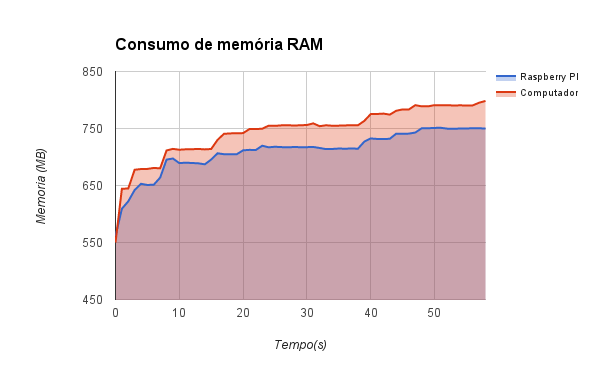
\includegraphics[scale=0.8]{Imagens/memoria}
\fonte{ Elaborado pelo autor}
\label{fig:memoria}
\end{figure}


Os dados apresentados na Figura \ref{fig:memoria} indicam que o \textit{Raspberry PI} utilizou em quase todo o período do teste uma quantidade menor de memória RAM que o computador, ambos executados nas mesmas condições. Durante a coleta desses dados utilizando o \textit{Raspberry PI}, o pico de memória foi de 751,2109 MB, enquanto o computador utilizou o teto de 798,3632 MB. Uma razoável diferença, levando em conta que o servidor antes de iniciar os testes utilizava entre 561,1641 MB e 549,8554 MB. 

Os dados coletados sobre o  uso de CPU mostram uma alternância no período dos testes, onde o \textit{Raspberry PI} apresentou um resultado mediano em relação ao computador.

\begin{figure}[!htb]
\centering
\caption{Porcentagem da utilização da CPU do servidor durante o uso do \textit{Raspberry PI} com \textit{thin client} e do computador como \textit{thin client}}
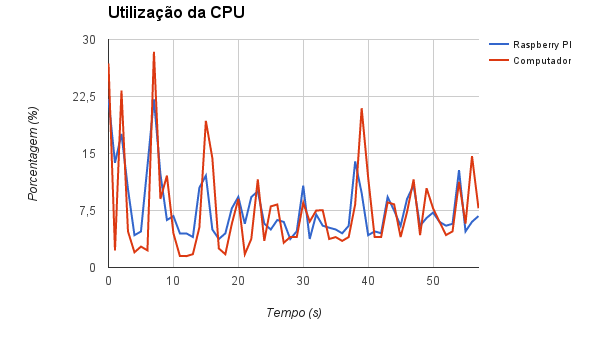
\includegraphics[scale=0.8]{Imagens/cpu_2}
\fonte{ Elaborado pelo autor}
\label{fig:cpu}
\end{figure}

A figura \ref{fig:cpu} ilustra a utilização da CPU durante o período dos testes três e quatro, onde é notado uma alternância entre o computador e o \textit{Raspberry PI}, no maior uso da CPU. O que indica um equilíbrio entre as ambas partes, já que a diferença é pequena do uso da CPU do servidor solicitada pelos \textit{thin clients}  no mesmo instante do teste.

A última informação coletada dos testes está relacionada a transferência de dados pela rede, tendo em vista que para um melhor desempenho no ambiente \textit{thin client}, a rede local não pode ficar sobrecarregada. Foi coletada a quantidade de dados transferidos pela interface do servidor no instante de iniciou os testes e outra coleta após o tempo limite dos testes. Sendo assim possível verificar a quantidade de dados enviados e recebidos da interface do servidor usada para a comunicação com os \textit{thin clients}.

A Figura \ref{fig:net} informa a quantidade de dados enviados e recebidos durante os testes. Lembrando que esses dados foram coletados do servidor.

\begin{figure}[!h]
\centering
\caption{Quantidade de dados transferidos pela rede durante o uso do \textit{Raspberry PI} com \textit{thin client} e do computador como \textit{thin client}}
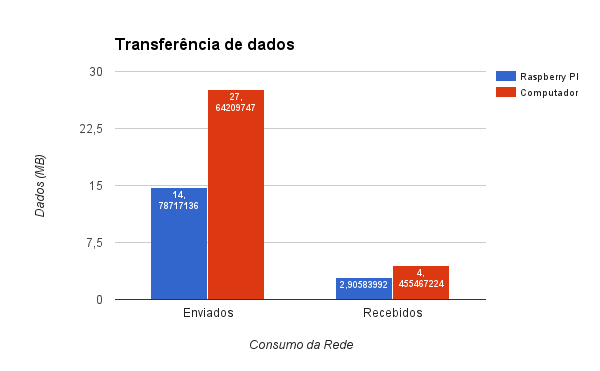
\includegraphics[scale=0.8]{Imagens/net}
\fonte{ Elaborado pelo autor}
\label{fig:net}
\end{figure}

\newpage
A Figura \ref{fig:net} apresenta bons resultados na utilização do \textit{Raspberry PI} como \textit{thin client}, necessitando apenas 14,78717136 MB de dados enviados  do servidor para executar os testes, isso é aproximadamente 53,47\% da quantidade solicitada pelo computador no modo \textit{thin client}. Os resultados continuam favoráveis ao \textit{Raspberry PI} nos dados que são enviados para o servidor, pois o ele enviou aproximadamente 65,21\% de dados que o computador.

As informações apresentadas na Figura \ref{fig:net} indicam que a utilização de \textit{Raspberry PI} no ambiente \textit{thin client} torna a rede local menos congestionada, transferindo menos dados e consequentemente ocupando menos largura de banda. 


% -----------------------------------------------------------------------------------------------------------
% Fim Análise e interpretação dos dados
% -----------------------------------------------------------------------------------------------------------

% -----------------------------------------------------------------------------------------------------------
% Finaliza o bookmark do PDF para que se inicie o bookmark na raiz e adiciona espaço de parte no Sumário
% -----------------------------------------------------------------------------------------------------------

\phantompart

% -----------------------------------------------------------------------------------------------------------
% Fim bookmark do PDF 
% -----------------------------------------------------------------------------------------------------------



% -----------------------------------------------------------------------------------------------------------
% Inseri Conclusão
% -----------------------------------------------------------------------------------------------------------

\chapter{Conclusão}

O \textit{Raspberry PI} modelo B usando o BerryTerminal, traz benefí	cios ao ambiente \textit{thin client}, como a diminuição da utilização dos recursos do servidor, a economia de energia utilizada e a economia para criação de infraestrutura de computadores. A sua utilização se enquadra no conceito mais profundo do TI verde, ou \textit{Green IT}, pois envolvendo uma nova estrutura de refrigeração e um melhor aproveitamento dos espaços físicos. 

O \textit{Raspberry PI} como um \textit{thin client}, consome também menos memória RAM a cerca de 23,55\% que um computador com \textit{thin client}. Essa diferença em um ambiente com várias maquinas possibilita a inserção de mais \textit{Raspberrys PI} do que computadores. Além de utilizar uma quantidade menor da banda em sua rede local.

Nos testes executados não foi possível acessar dispositivos de armazenamento conectados via USB no \textit{Raspberry PI}, dificultando a transferência dos dados utilizados no ambiente \textit{thin client}. Uma alternativa que viabiliza essa transferência é a conexão do dispositivo no servidor, algo que não é muito aconselhado e muitas vezes não acessível aos usuários.

A usabilidade do \textit{Raspberry PI} como \textit{thin client} gerou resultados que não são motivos de elogio, já que ele teve um mal desempenho na execução de vídeos e dificuldades de na exibição da tela como a perda de algumas transições.

No geral, os resultados da comparação entre o computador e o \textit{Raspberry PI}, ambos como \textit{thin client}, foram neutros já que o \textit{Raspberry PI} teve um melhor desempenho na utilização dos recursos e o computador desempenhou um ótimo papel usabilidade e na fluidez da utilização. Deixando o resultado equilibrado. Mas como o \textit{Raspberry PI} possui outras vantagens, como preço e a economia de energia, tanto diretamente quanto indiretamente. Deixando o \textit{Raspberry PI} com um saldo positivo.

Então é correto afirmar que o \textit{Raspberry PI} é uma boa opção de \textit{thin client}, mas vale ressaltar que é preciso verificar qual a finalidade do ambiente \textit{thin client}, pois o \textit{Raspberry PI} com o BerryTerminal não é aconselhado em ambientes onde ocorre edição de vídeos ou imagens. Mas altamente recomentado em ambientes onde se utiliza nuvens para o armazenamento dos dados.

Para a obtenção de resultados mais precisos, é necessário avançar com a pesquisa produzindo outros testes com diferentes modelos de \textit{Raspberry PI} para verificar se os problemas encontrados, estão presentes apenas no modelo usado, ou não. Também buscar outros softwares que permitam que o \textit{Raspberry PI} seja um \textit{thin client}, semelhante ao que o BerryTerminal faz.

Outro projeto interessante é, verificar a quantidade de \textit{thin clients} suportando por uma rede local utilizando o cabo RJ-45. Ou realização de testes para determinar o desempenho de uma thin client a grande distância, determinado até que distancia o Raspberry PI como thin client traz bons resultados.  





% -----------------------------------------------------------------------------------------------------------
% Fim Conclusão
% -----------------------------------------------------------------------------------------------------------



% -----------------------------------------------------------------------------------------------------------
% ELEMENTOS PÓS-TEXTUAIS
% -----------------------------------------------------------------------------------------------------------

\postextual

% -----------------------------------------------------------------------------------------------------------
% Fim ELEMENTOS PÓS-TEXTUAIS
% -----------------------------------------------------------------------------------------------------------



% -----------------------------------------------------------------------------------------------------------
% Inseri Referências bibliográficas
% -----------------------------------------------------------------------------------------------------------

\bibliography{REFERENCIAS}

% -----------------------------------------------------------------------------------------------------------
% Fim Referências bibliográficas
% -----------------------------------------------------------------------------------------------------------

% ---
% Inicia os apêndices
% ---
\begin{apendicesenv}

% Imprime uma página indicando o início dos apêndices
\partapendices

\chapter{Script para criar servidor LTSP}
\label{script:servidor}
Script também está acessível no repositório público do trabalho disponível em	 \url{https://github.com/FelipeLimaM/thin-client-raspberry-pi-tcc/tree/master/thin_client/build_server}

\begin{verbatim}
build_server.sh

#!/bin/bash

# author Felipe Lima Morais - Graduando de Ciência da Computação
CHOICE_INTERFACE_DIR=/etc/default/isc-dhcp-server
CONF_INTERFACE_DIR=/etc/network/interfaces

NEW_CONF=ConfInterface
NEW_CONF_BAK=ConfInterface.backup

if [[ $EUID -ne 0 ]]; then
    echo "This script must be run as root" #1>&2
else
    INSTALL_PACKAGE=ltsp-server-standalone
    
    clear
    echo " update packages"
    sleep 1
    sudo apt-get install update

    clear
    echo " upgrade of packages"
    sleep 1
    sudo apt-get upgrade -y 

    clear
    echo " download/install package ltsp-server-standalone install"
    sleep 2
    sudo apt-get install $INSTALL_PACKAGE -y

	sudo apt-get install gnome-session-fallback -y
	sudo/usr/lib/lightdm/lightdm-set-defaults -s gnome-fallback


    if ((1<<32)); then
        echo your 64bits system
        ltsp-build-client --arch="i386" 
    else
        echo you 32bits system
        ltsp-build-client
    fi
	clear
	# ALTER  /etc/default/isc-dhcp-server
	connect=$(ifconfig |  grep -E encap | awk -F 'Link' '{print $1 }' \
	| awk -F '$' '{print $1 }')
	echo "choose the interface to the LTSP environment?"
	echo ""	
	select result in $connect
	do
		if [ -n "$result" ]; then	
			
			INTERFACE=$result
			sed -i 's/INTERFACES\=.*/INTERFACES\=\"'$result'\"/g' $CHOICE_INTERFACE_DIR	
			break
		fi
	done

	# BACKUP / ALTER  /etc/network/interfaces
	
	(cat $NEW_CONF) > $NEW_CONF_BAK

	sed -i 's/???/'$result'/g' $NEW_CONF

	(cat $NEW_CONF) >> $CONF_INTERFACE_DIR

	(cat $NEW_CONF_BAK) > $NEW_CONF

	rm $NEW_CONF_BAK
	
	clear
	echo "click ENTER to restart the system"
	read
	sudo reboot	
	
fi
--
\end{verbatim}

\begin{verbatim}
ConfInterface

auto ???
iface ??? inet static
        address 192.168.0.1
        network 192.168.0.0
        netmask 255.255.255.0
        broadcast 192.168.0.255
--
\end{verbatim}


\chapter{Scripts para coletar dados do servidor}
\label{script:GetDataServer}
Os Scripts também são acessíveis no repositório público do trabalho disponível em \url{https://github.com/FelipeLimaM/thin-client-raspberry-pi-tcc/tree/master/thin_client/test}

\begin{verbatim}
get_data_server.sh

#!/bin/bash

file_memory='memory'
file_cpu='cpu'
 
start_time=`date -d "10/19/2015 23:50" +%s`
end_time=`date -d "10/19/2015 23:51" +%s`

if [[ $EUID -ne 0 ]]; then
    echo "This script must be run as root" #1>&2
else
	echo "wait.."
	bash collect_data_memory.sh & #start collection
	aux=$(cat exec.wa)
	pid_memory=`expr $aux - 2`
	echo "pid_memory $pid_memory"

	bash collect_data_cpu.sh & #start collection
	aux=$(cat exec.wa)
	pid_cpu=`expr $aux - 2`
	echo "pid_cpu $pid_cpu"

	sleep $(expr $start_time - `date +%s`) #start time to script
	echo "go go $(date)"

	start_RX=$(ifconfig eth0 | grep 'bytes'|\
	 awk -F "(:|\()" '{print $2}') #get RX initial
	start_TX=$(ifconfig eth0 | grep 'bytes'|\
	 awk -F "(:|\()" '{print $4}') #get TX initial
	start_memory=$(free -kt | grep Mem |\
	 awk '{print expr ($3 - ($6 + $7))}') #get memory initial
	start_cpu=$(cat <(grep 'cpu ' /proc/stat) <(sleep 1 && grep 'cpu ' /proc/stat) |\
	 awk -v RS="" '{print ($13-$2+$15-$4)*100/($13-$2+$15-$4+$16-$5)}') #get cpu initial

	rm $file_memory
	rm $file_cpu

	while [ true ]; do
		echo "loop"
		sleep 1
		if [ $(date +%s) -ge $end_time ]; then
			break;
		fi
	done
	if [ -a test_cpu ]; then rm test_cpu; fi
	if [ -a test_memory ]; then rm test_memory; fi
	(cat $file_memory)>test_memory
	(cat $file_cpu)>test_cpu
	end_RX=$(ifconfig eth0 | grep 'bytes'| awk -F "(:|\()" '{print $2}') #transfer net
	end_TX=$(ifconfig eth0 | grep 'bytes'| awk -F "(:|\()" '{print $4}') #transfer net

	#solution data (net)
	net_RX=`expr $end_RX - $start_RX`
	net_TX=`expr $end_TX - $start_TX`

	#solution data (memory)
	memory_used=0
	$start_memory
	memory_used=(`python -c "print (max([float(line.rstrip('\n'))\
	 for line in open('test_memory')]) - float($start_memory))/1024"`)

	#solution data (CPU)
	cpu_used=0
	cpu_max=(`python -c "print max([float(line.rstrip('\n'))\
	 for line in open('test_cpu')])"`)

	date
	echo -e "memory used \t $memory_used"
	echo -e "trafic send \t $net_RX" 
	echo -e "trafic reciv \t $net_TX" 
	echo -e "cpu upper \t $cpu_max"
fi
--
\end{verbatim}



\begin{verbatim}
collect_data_cpu.sh

#!/bin/bash

file='cpu'

if [ -a $file ]; then rm $file; fi
(echo $BASHPID)>exec.wa

while (cat <(grep 'cpu ' /proc/stat) <(sleep 1 && grep 'cpu ' /proc/stat) |\
 awk -v RS="" '{print ($13-$2+$15-$4)*100/($13-$2+$15-$4+$16-$5)}')>>$file; do 
    i=0; 
done
--
\end{verbatim}


\begin{verbatim}
collect_data_memory.sh

#!/bin/bash

file='memory'

if [ -a $file ]; then rm $file; fi 
(echo $BASHPID)>exec.wa

while (free -kt | grep Mem | awk '{print expr ($3 - ($6 + $7))}')>>$file; do 
    sleep 1
done
--
\end{verbatim}


\chapter{Script que sumilar a utilização de um cliente}
\label{script:ExecClient}
Script também está acessível no repositório público do trabalho disponível em	 \url{https://github.com/FelipeLimaM/thin-client-raspberry-pi-tcc/blob/master/thin_client/test/ltsp_client.sh}

\begin{verbatim}
ltsp_client.sh

#!/bin/bash

arr=("firefox" "libreoffice --writer" "rhythmbox" "libreoffice --calc"\
 "/usr/games/gnome-sudoku" "libreoffice --draw" "libreoffice --calc"\
 "/usr/games/sol"); 

temp=(3 5 2 6 1 0 4 3 2 8 4 1 4 5 1 6 3 1 6 7 3 1 5 2 5);

n=`expr ${#arr[@]} - 1`

start_time=`date -d "10/19/2015 23:50" +%s`
end_time=`date -d "10/19/2015 23:51" +%s`

sleep $(expr $start_time - `date +%s`) #start time to script

while [ true ]; do
	
	for i in `seq 0 $n`; do
		${arr[$i]} &
		sleep ${temp[$i]}
	done

	if [ $(date +%s) -ge $end_time ]; then
		break;
	fi
done
--
\end{verbatim}




\end{apendicesenv}
% ---


% ----------------------------------------------------------
% Anexos
% ----------------------------------------------------------

% ---
% Inicia os anexos
% ---
%\begin{anexosenv}

% Imprime uma página indicando o início dos anexos
%\partanexos

% ---

%\end{anexosenv}

%---------------------------------------------------------------------
% INDICE REMISSIVO
%---------------------------------------------------------------------
\phantompart
\printindex
%---------------------------------------------------------------------

\end{document}
